\section{载流子的扩散运动}
在\xref{sec:载流子的漂移运动}中,我们讨论了载流子在电场作用下的漂移运动,在本节,我们将讨论载流子在浓度梯度作用下的\uwave{扩散运动}(Diffusion)。那么,扩散为什么要放在本章讨论?扩散运动和非平衡载流子之间有什么关系吗?扩散的根本在于浓度差,而产生不均匀的载流子分布的最简单的方法是,使半导体的一侧接受均匀光照,半导体在顺光侧将会产生大量非平衡载流子,半导体的内部和背光侧则几乎没有任何非平衡载流子,由此就可以形成浓度梯度,发生扩散。

简洁起见,我们考虑一维情况,即假定非平衡载流子的浓度只随$x$变化,记作$\delt{p}(x)$,那么浓度梯度就可以记为$\dv*{\delt{p}}{x}$。通常,我们将单位时间内通过单位面积的粒子数称为\uwave{扩散流密度}(Diffusion Flux)。\uwave{菲克扩散定律}(Fick's Laws of Diffusion)指出,\empx{扩散流密度总是与粒子的浓度的负梯度成正比},若用$S_\text{p}$表示空穴扩散流密度,而用$D_\text{p}$表示空穴扩散系数,则有
\setpeq{载流子的扩散运动}
\begin{BoxLaw}[菲克扩散定律]
    扩散流密度,正比于浓度负梯度
    \begin{Equation}&[1]
        S_\text{p}=-D_\text{p}\dv{\delt{p}}{x}
    \end{Equation}
\end{BoxLaw}
我们会问,为什么是空穴?非平衡载流子不是既有空穴又有电子的吗?这是因为根据\xref{sec:非平衡载流子的产生与复合}的讨论,当我们在杂质半导体中注入时,实际上,主要起作用的是非平衡少数载流子,换言之
\begin{itemize}
    \item N型半导体只需考虑非平衡空穴$\delt{p}$,即空穴的扩散运动。
    \item P型半导体只需考虑非平衡电子$\delt{n}$,即电子的扩散运动。
\end{itemize}
这里,我们以N型半导体为例,故只考虑$\delt{p}$,而相关结论很容易可以推广至P型和$\delt{n}$。

现在让我们将\xrefpeq{1}两端对$x$求导
\begin{Equation}&[2]
    D_\text{p}\dv[2]{\delt{p}(x)}{x}=-\dv{S_\text{p}(x)}{x}
\end{Equation}
如果这是三维情况,先前$\dv*{\delt{p}}{x}$是求梯度,而此步的求导就变成求散度了,因而\xrefpeq{2}右端的意义即空穴扩散流密度的汇,而什么又会构成空穴扩散流密度的汇呢?答案,就是载流子的复合,这里的汇即单位时间单位体积内因复合消失的空穴数$\delt{p}(x)/\tau$,因此就有
\begin{Equation}
    D_\text{p}\dv[2]{\delt{p}(x)}{x}=\frac{\delt{p}(x)}{\tau}
\end{Equation}
这就是一维稳定扩散情况下,非平衡少数载流子所遵循的扩散方程,称为稳态扩散方程。

\begin{BoxEquation}[稳态扩散方程]
    非平衡少数载流子的浓度$\delt{p}$,遵循以下稳态扩散方程
    \begin{Equation}&[A]
        D_\text{p}\dv[2]{\delt{p}}{x}=\frac{\delt{p}}{\tau}
    \end{Equation}
    其通解为
    \begin{Equation}&[B]
        \delt{p}(x)=A\exp(-\frac{x}{L_\text{p}})+B\exp(\frac{x}{L_\text{p}})\qquad L_\text{p}=\sqrt{D_\text{p}\tau}
    \end{Equation}
\end{BoxEquation}
稳态扩散方程是一个标准的二阶微分方程,故这里我们不再具体分析其通解的求解过程。而接下来,我们愿意讨论$\delt{p}$的通解在两种特定条件下的具体形式,即$\delt{p}$的具体分布规律?

\subsection{样品足够厚}
\begin{BoxFormula}[样品足够厚时非平衡载流子的浓度分布]
    样品足够厚时,非平衡载流子的浓度可以表示为
    \begin{Equation}
        \delt{p}(x)=(\delt{p})_0\exp(-\frac{x}{L_\text{p}})
    \end{Equation}
    其中$(\delt{p})_0$是样品光照一端的非平衡载流子浓度。
\end{BoxFormula}
\begin{Proof}
    设样品足够厚,非平衡载流子到达样品的另外一端时已经几乎复合殆尽了,即
    \begin{Equation}&[1]
        \delt{x}\to\infty\qquad\delt{p}\to 0
    \end{Equation}
    因此,正指数项是不被允许存在的,故\xrefpeq[稳态扩散方程]{B}中的$B=0$,即
    \begin{Equation}&[2]
        \delt{p}(x)=A\exp(-\frac{x}{L_\text{p}})
    \end{Equation}
    而在样品受光照的一端,非平衡载流子浓度为定值
    \begin{Equation}&[3]
        \delt{p}(0)=(\delt{p})_0
    \end{Equation}
    这表明$A$其实就是$(\delt{p})_0$,因而\xrefpeq{2}
    \begin{Equation}*
        \delt{p}(x)=(\delt{p})_0\exp(-\frac{x}{L_\text{p}})\qedhere
    \end{Equation}
\end{Proof}

\xref{fml:样品足够厚时非平衡载流子的浓度分布}指出,非平衡少数载流子从光照表面的$(\delt{p})_0$开始,向内部依负指数规律衰减。而很明显的是,这里$L_\text{p}=\sqrt{D_\text{p}\tau}$代表非平衡载流子在扩散过程中不断复合,浓度减小至原有浓度的$1/\e$时的扩散距离,即$\delt{p}(x+L_\text{p})=\delt{p}(x)/\e$。而除此之外,通过下面的推导亦可以证明,其实$L_\text{p}$还是非平衡载流子深入样品的平均距离,称为\uwave{扩散长度}(Diffusion Length)。
\begin{Equation}
    \bar{x}=\frac{\Int[0][\infty]x\delt{p}(x)\dx}{\Int[0][\infty]\delt{p}(x)\dx}=
    \frac{\Int[0][\infty]x\exp(-x/L_\text{p})\dx}{\Int[0][\infty]\exp(-x/L_\text{p})\dx}=L_\text{p}
\end{Equation}

这里的数学与先前\xrefeq{寿命即平均生存时间}是完全相同的。

\begin{BoxFormula}[样品足够厚时非平衡载流子的扩散流密度]
    样品足够厚时,非平衡载流子的扩散流密度可以表示为
    \begin{Equation}
        S_\text{p}(x)=\frac{D_\text{p}}{L_\text{p}}\delt{p(x)}
    \end{Equation}
\end{BoxFormula}
\begin{Proof}
    根据\fancyref{law:菲克扩散定律}
    \begin{Equation}
        S_\text{p}(x)=-D_\text{p}\dv{\delt{p}}{x}
    \end{Equation}
    根据\fancyref{fml:样品足够厚时非平衡载流子的浓度分布}
    \begin{Equation}
        S_\text{p}(x)=-D_\text{p}\dv{x}\qty[(\delt p_0)\exp(-\frac{x}{L_\text{p}})]
    \end{Equation}
    计算导数
    \begin{Equation}*
        S_\text{p}(x)=\frac{D_\text{p}}{L_\text{p}}(\delt{p_0})\exp(-\frac{x}{L_\text{p}})=\frac{D_\text{p}}{L_\text{p}}\delt{p}(x)\qedhere
    \end{Equation}
\end{Proof}
\xref{fml:样品足够厚时非平衡载流子的扩散流密度}指出,样品足够厚时,非平衡载流子的扩散流密度正比于非平衡载流子浓度。

\subsection{样品厚度一定}
\begin{BoxFormula}[样品厚度一定时非平衡载流子的浓度分布]
    样品厚度一定时,非平衡载流子的浓度可以表示为
    \begin{Equation}
        \delt{p}(x)=(\delt{p})_0\frac{\sinh(W-x/L_\text{p})}{\sinh(W/L_\text{p})}
    \end{Equation}
    其中$(\delt{p})_0$是样品光照一端的非平衡载流子浓度,而$W$为样品厚度。

    样品厚度$W$若远小于扩散长度$L$,即当$W\ll L$时,有近似式
    \begin{Equation}
        \delt{p}(x)=(\delt{p})_0\qty(1-\frac{x}{W})
    \end{Equation}
\end{BoxFormula}

\begin{Proof}
    设样品厚度为$W$,并且在样品另一端设法将非平衡少数载流子全部引出。

    因此,这里的边界即
    \begin{Equation}
        \delt{p}(0)=(\delt{p})_0\qquad
        \delt{p}(W)=0
    \end{Equation}
    代入\xrefpeq[稳态扩散方程]{B}
    \begin{Equation}
        A+B=(\delt{p})_0\qquad
        A\exp(-\frac{W}{L_\text{p}})+
        B\exp(\frac{W}{L_\text{p}})=0
    \end{Equation}
    这是一个关于$A,B$的二元一次方程,改写为矩阵形式
    \begin{Equation}
        \begin{pmatrix}
            1&1\\
            \exp(-W/L_\text{p})&
            \exp(W/L_\text{p})
        \end{pmatrix}
        \begin{pmatrix}
            A\\
            B
        \end{pmatrix}=
        \begin{pmatrix}
            (\delt{p})_0\\
            0
        \end{pmatrix}
    \end{Equation}
    计算几个关键的行列式
    \begin{Gather}*[15pt]
        D=
        \begin{vmatrix}
            1&1\\
            \exp(-W/L_\text{p})&
            \exp(W/L_\text{p})
        \end{vmatrix}=
        \exp(W/L_\text{p})-\exp(-W/L_\text{p})\\
        D_A=
        \begin{vmatrix}
            (\delt{p})_0&1\\
            0&\exp(W/L_\text{p})
        \end{vmatrix}=
        (\delt{p})_0\exp(W/L_\text{p})\\
        D_B=
        \begin{vmatrix}
            1&(\delt{p})_0\\
            \exp(-W/L_\text{p})&0\\
        \end{vmatrix}=
        -(\delt{p})_0\exp(-W/L_\text{p})
    \end{Gather}
    由此即可得到
    \begin{Gather}[15pt]
        A=\frac{D_A}{D}=\frac{(\delt{p})_0\exp(W/L_\text{p})}{\exp(W/L_\text{p})-\exp(-W/L_\text{p})}\\
        B=\frac{D_B}{B}=\frac{-(\delt{p})_0\exp(-W/L_\text{p})}{\exp(W/L_\text{p})-\exp(-W/L_\text{p})}
    \end{Gather}
    根据\xrefpeq[稳态扩散方程]{B}
    \begin{Equation}
        \delt{p}(x)=A\exp(-\frac{x}{L_\text{p}})+B\exp(\frac{x}{L_\text{p}})
    \end{Equation}
    即得
    \begin{Equation}
        \delt{p}(x)=(\delt{p})_0\frac{\exp[(W-x)/L_\text{p}]-\exp[-(W-x)/L_\text{p}]}{\exp(W/L_\text{p})-\exp(-W/L_\text{p})}
    \end{Equation}
    我们可以使用双曲正弦简化
    \begin{Equation}
        \delt{p}(x)=(\delt{p})_0\frac{\sinh(W-x/L_\text{p})}{\sinh(W/L_\text{p})}
    \end{Equation}
    近似式亦不难证明
    \begin{Equation}
        \delt{p}(x)=(\delt{p})_0\frac{W-x/L_\text{p}}{W/L_\text{p}}=(\delt{p})_0\frac{W-x}{W}=(\delt{p})_0\qty(1-\frac{x}{W})
    \end{Equation}
    近似的关键在于利用双曲正弦在$t\to 0$时的等价无穷小$\sinh(t)\sim t$的特性。
\end{Proof}

通过\xref{fig:非平衡载流子的浓度分布},我们可以很直观的看到,在样品厚度有限时,载流子浓度$\delt{p}$会在$x=W$处降低至零,并且,样品厚度$W$越大则$\delt{p(x)}$的分布曲线越接近于样品足够厚时的曲线(这说明我们的理论是连续过渡的),同时,样品厚度$W<L_\text{p}$较小时,$\delt{p}$的分布逐渐趋近于线性。

\begin{Figure}[非平衡载流子的浓度分布]
    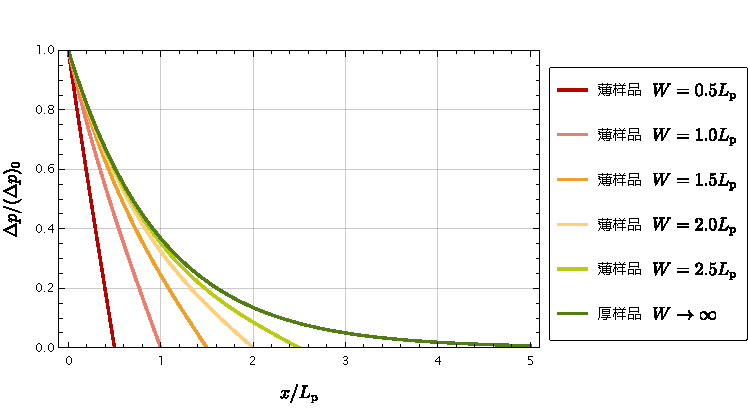
\includegraphics[scale=0.95]{Mathematica/output/DeltP.pdf}
\end{Figure}

\subsection{扩散电流密度}
在\xref{subsec:样品足够厚}和\xref{subsec:样品厚度一定}中,我们详细讨论了不同情况下,非平衡载流子的浓度$\delt{n},\delt{p}$应当如何表示,这为我们依据\fancyref{law:菲克扩散定律}具体计算扩散流密度$S_\text{n},S_\text{p}$提供了依据,考虑到扩散流密度正比于浓度的负梯度。不过在本小节,我们实际上并不关心$\delt{n},\delt{p}$的具体形式。前面讨论的都是扩散流密度,但是实践中更有价值的是扩散导致的电流有多少?很显然,扩散电流密度$J_\text{n},J_\text{p}$应当正比于扩散流密度$S_\text{n},S_\text{p}$,比例系数为载流子的电荷量$\mp q$
\begin{Equation}
    J_\text{n}=-qS_\text{n}\qquad
    J_\text{p}=qS_\text{p}
\end{Equation}
在上式中代入\fancyref{law:菲克扩散定律},这就是本小节要掌握的全部了。
\begin{BoxFormula}[扩散电流密度]
    半导体中,扩散电流密度满足
    \begin{Equation}
        J=J_\text{n}+J_\text{p}=qD_\text{n}\dv{\delt{n}}{x}-qD_\text{p}\dv{\delt{p}}{x}
    \end{Equation}
    其中,$\delt{n},\delt{p}$分别代表非平衡电子和空穴的浓度,$D_\text{n},D_\text{p}$为电子和空穴的扩散系数。
\end{BoxFormula}